\documentclass[letterpaper,journal]{IEEEtran}
\usepackage{cite}
\usepackage{amsmath,amsfonts,amssymb}
\usepackage{array}
\usepackage[caption=false,font=normalsize,labelfont=sf,textfont=sf]{subfig}
\usepackage{textcomp}
\usepackage{stfloats}
\usepackage{url}
\usepackage{graphicx}
\usepackage{balance}
\hyphenation{Koop-man pre-dic-tive}
\def\BibTeX{{\rm B\kern-.05em{\sc i\kern-.025em b}\kern-.08em
    T\kern-.1667em\lower.7ex\hbox{E}\kern-.125emX}}

\newtheorem{assumption}{Assumption}
\newtheorem{proposition}{Proposition}
\newtheorem{remark}{Remark}

\begin{document}

\title{Tube-Tightened Bilinear Koopman Model Predictive Guidance for Impact-Angle-Constrained Interception Without Prescribed Impact Time}

\author{Qiuya Li
\thanks{This manuscript is a working draft prepared from the current Koopman guidance workspace. The author affiliation and funding information should be completed before submission.}}

\markboth{Working Draft, Koopman Guidance Manuscript, 2026}%
{Li: Bilinear Koopman Model Predictive Guidance Without Prescribed Impact Time}

\maketitle

\begin{abstract}
This paper investigates a Koopman-operator-based model predictive guidance method for planar stationary-target interception with an impact-angle constraint but without a prescribed impact-time constraint. Removing the fixed terminal-time requirement changes the guidance objective from scheduled interception to capture with a desired terminal direction, which is less restrictive and more consistent with reachable-set limitations observed in fixed-time tuning. The development separates the unconstrained guidance core from the angle-constrained terminal task. It is first shown that the ideal Cartesian acceleration-controlled stationary-target model admits an exact finite-dimensional continuous-time bilinear Koopman representation under the constant-speed assumption. A geometric terminal-error model is then constructed in the desired impact-angle frame, where along-track progress, cross-track displacement, and terminal heading error provide the regulated prediction outputs. Based on this structure, a task-oriented bilinear extended dynamic mode decomposition predictor is identified from sampled trajectories and embedded into a sequential convex Koopman model predictive controller with a first-order autopilot state, input-difference regularization, terminal slack variables, and validation-data residual-tube tightening. Numerical simulations show that the proposed angle-only design satisfies a 5 m capture-radius requirement for the nominal 30$^\circ$ case, achieving a 3.048 m miss distance and a $0.109^\circ$ impact-angle error, while the speed-perturbed stress case also remains inside the capture set with a 4.150 m miss distance and a $0.121^\circ$ angle error. Additional nominal tests satisfy 10 m capture-radius requirements for 30$^\circ$ and 45$^\circ$ impact-angle commands. Acceleration-rate scans show that moderate command-smoothing constraints can improve the capture result, whereas large-angle cases expose the remaining reachable-envelope and solver-reliability limitations. These results support a bounded claim: bilinear Koopman-MPC is a useful QP-based predictive-guidance framework for nominal impact-angle-constrained interception when impact time is treated as an outcome rather than as a hard command.
\end{abstract}

\begin{IEEEkeywords}
Koopman operator, model predictive guidance, impact-angle constraint, residual tube, bilinear predictor, angle-only guidance.
\end{IEEEkeywords}

\section{Introduction}
\IEEEPARstart{T}{erminal} guidance often requires a pursuer not only to reduce miss distance, but also to approach the target from a prescribed direction. Impact-angle guidance is therefore important in planar interception, precision engagement, and terminal path-shaping problems. Unlike simultaneous impact-time and impact-angle guidance, the angle-only problem does not require the pursuer to arrive at a specified clock time. The controller may instead use the available maneuvering authority to shape the trajectory and let the actual impact time emerge from the closed-loop motion.

Model predictive control (MPC) is attractive for angle-constrained guidance because it can handle terminal tolerances, acceleration bounds, and command-smoothing requirements in a single optimization problem. Direct nonlinear MPC, however, can be too expensive or unreliable for repeated terminal-guidance updates. Koopman operator methods offer an alternative route: nonlinear dynamics are embedded in a lifted observable space so that prediction becomes approximately linear or structured bilinear. Koopman predictors have been used in MPC for nonlinear systems and in Koopman-operator-based integrated guidance and control for high-speed missiles \cite{korda2018mpc,bevanda2021kodm,zhou2024klmpc}. This paper follows that predictor-then-MPC logic, but narrows the terminal task to impact-angle-constrained capture without enforcing a scheduled impact time.

The main technical issue is that interception is not a regulation equilibrium in the original Cartesian relative coordinates. At capture, the relative position is near zero, but the velocity does not vanish. A useful predictive-guidance coordinate must therefore describe terminal geometry rather than regulate the original position state as a static equilibrium. For the angle-only problem, we use an impact-frame terminal-error state that contains along-track progress, cross-track displacement, and heading error. The along-track component is used as a progress and terminal-position reference, but not as a hard clock-time command.

The main contributions are summarized as follows.
\begin{enumerate}
    \item A finite-dimensional continuous-time bilinear Koopman representation is derived for the unconstrained constant-speed stationary-target guidance core in Cartesian relative coordinates. This result explains why a bilinear lifted predictor is structurally better matched to the control-affine guidance dynamics than a purely linear input predictor.
    \item The terminal guidance task is reformulated as impact-angle-constrained capture in a desired-impact-frame error coordinate. The formulation removes the prescribed impact-time constraint while retaining a terminal target for cross-track error, heading error, and near-target capture.
    \item A data-driven sequential convex bilinear Koopman-MPC controller is constructed with measured-predicted lifted-state interpolation, move and acceleration-difference regularization, terminal slack variables, and validation-data residual-tube tightening.
    \item Numerical simulations report nominal and stress angle-only capture results, prediction-accuracy diagnostics, acceleration-rate constraint scans, and large-angle boundary cases. The results are presented as evidence for nominal angle-only guidance rather than as evidence for fixed-time interception.
\end{enumerate}

The remainder of this paper is organized as follows. Section II gives the planar engagement model and the basic interception objective. Section III develops the basic exact-bilinear Koopman predictive guidance law. Section IV extends the formulation to impact-angle-constrained guidance. Section V describes the data-driven bilinear Koopman-MPC implementation used in simulation. Section VI reports numerical results, and Section VII concludes the paper.

\section{Planar Engagement Model and Basic Interception Problem}

\subsection{Relative Motion Model}
Consider a stationary target at the origin and a pursuer moving at constant nominal speed $V>0$ in a planar engagement. Let
\begin{equation}
    r=\begin{bmatrix}r_x&r_y\end{bmatrix}^T,\qquad
    \gamma\in\mathbb R
\end{equation}
denote the relative position and flight-path angle, respectively. The normalized lateral-acceleration command is
\begin{equation}
    u=\frac{A}{A_{\max}},\qquad |u|\le 1 .
\end{equation}
The ideal acceleration-controlled guidance core is
\begin{equation}
    \dot r_x=-V\cos\gamma,\qquad
    \dot r_y=-V\sin\gamma,\qquad
    \dot\gamma=\frac{A_{\max}}{V}u .
    \label{eq:cartesian_model_angle_only}
\end{equation}
The closed-loop simulations pass the optimized command $u_c$ through a first-order autopilot,
\begin{equation}
    \dot\gamma=\frac{A_{\max}}{V}u_a,\qquad
    \tau_a\dot u_a=-u_a+u_c,\qquad |u_c|\le1 ,
    \label{eq:autopilot_angle_only}
\end{equation}
where $u_a$ is the actual normalized lateral acceleration. The ideal model \eqref{eq:cartesian_model_angle_only} is recovered when $u_a=u_c=u$.

\begin{assumption}
The target is stationary, the pursuer speed is constant within each case, the command is piecewise constant and bounded, and the engagement is considered before the singular intercept instant. The heading angle is treated as an unwrapped real variable when differentiability is required.
\end{assumption}

\subsection{Basic Capture Objective}
Before imposing an impact-angle requirement, the basic interception task is to drive the relative position into a capture ball around the target,
\begin{equation}
    \min_t \|r(t)\|\le r_c ,
    \label{eq:basic_capture_objective}
\end{equation}
while respecting acceleration limits. In the receding-horizon implementation this objective is represented by a terminal position penalty and a softened terminal tolerance on the predicted relative position. This basic problem clarifies the Koopman prediction model and input-constrained MPC law before terminal angle shaping is added.

\section{Basic Exact-Bilinear Koopman Predictive Guidance Law}

\subsection{Exact Bilinear Koopman Prediction Model}
For a controlled nonlinear system
\begin{equation}
    \dot x=f_0(x)+u f_1(x),
\end{equation}
the controlled Koopman generator acting on a smooth observable $g$ is
\begin{equation}
    \mathcal L_u g(x)=\nabla g(x)^T(f_0(x)+u f_1(x))
    =\mathcal L_0g(x)+u\mathcal L_1g(x).
\end{equation}
This expression is a generator representation for a controlled system. It should not be interpreted as a single autonomous Koopman operator independent of the input.

\paragraph{Exact continuous-time bilinear lift:}
Let the core state be
\begin{equation}
    x_c=\begin{bmatrix}r_x&r_y&\gamma\end{bmatrix}^T .
\end{equation}
For \eqref{eq:cartesian_model_angle_only}, define the analytic lifted state
\begin{equation}
    z_c=\psi_c(x_c)=
    \begin{bmatrix}
    1&r_x&r_y&\gamma&\cos\gamma&\sin\gamma
    \end{bmatrix}^T .
    \label{eq:exact_lift_angle_only}
\end{equation}
The observable span generated by \eqref{eq:exact_lift_angle_only} is invariant under $\mathcal L_0$ and $\mathcal L_1$ because
\begin{equation}
    \mathcal L_0 r_x=-V\cos\gamma,\qquad
    \mathcal L_0 r_y=-V\sin\gamma ,
\end{equation}
and
\begin{equation}
\begin{aligned}
    \mathcal L_1 \gamma&=\frac{A_{\max}}{V},\\
    \mathcal L_1 \cos\gamma&=-\frac{A_{\max}}{V}\sin\gamma,\\
    \mathcal L_1 \sin\gamma&=\frac{A_{\max}}{V}\cos\gamma .
\end{aligned}
\end{equation}
Therefore
\begin{equation}
    \dot z_c=A_{0c}z_c+uB_{1c}z_c ,
    \label{eq:exact_bilinear_angle_only}
\end{equation}
where the nonzero entries are
\begin{equation}
    A_{0c}(2,5)=-V,\quad A_{0c}(3,6)=-V,
\end{equation}
\begin{equation}
\begin{aligned}
    B_{1c}(4,1)&=\frac{A_{\max}}{V},\\
    B_{1c}(5,6)&=-\frac{A_{\max}}{V},\\
    B_{1c}(6,5)&=\frac{A_{\max}}{V}.
\end{aligned}
\end{equation}

\begin{proposition}
Under Assumption 1, the planar stationary-target guidance core \eqref{eq:cartesian_model_angle_only} admits the exact finite-dimensional continuous-time bilinear Koopman representation \eqref{eq:exact_bilinear_angle_only} on the observable space spanned by \eqref{eq:exact_lift_angle_only}.
\end{proposition}

\begin{remark}
The exact continuous-time bilinear representation is a structural result for the ideal core. Under zero-order-hold input, the exact discrete lifted map is $z_{c,k+1}=\exp(T_s(A_{0c}+u_kB_{1c}))z_{c,k}$, which depends nonlinearly on $u_k$. The online predictor below is therefore a task-oriented finite-dimensional approximation on the sampled operating domain.
\end{remark}

\subsection{Receding-Horizon Basic Interception Formulation}
At sampling instant $k$, the basic Koopman predictive controller propagates the lifted state over a horizon $N$ and optimizes the future normalized acceleration sequence
\begin{equation}
    \mathbf U_k=[u_{0|k},u_{1|k},\ldots,u_{N-1|k}]^T .
\end{equation}
For the exact core model, a zero-order-hold prediction can be written as
\begin{equation}
    z_{i+1|k}=\Phi(u_{i|k})z_{i|k},\qquad
    \Phi(u)=\exp(T_s(A_{0c}+uB_{1c})) .
\end{equation}
For online quadratic programming, this prediction is locally approximated by the bilinear or linearized lifted models described in Sections III-D and V. The basic output is the relative position extracted from the lifted state,
\begin{equation}
    y^b_{i|k}=C_r z_{i|k}=
    \begin{bmatrix}r_{x,i|k}&r_{y,i|k}\end{bmatrix}^T .
\end{equation}
The terminal reference is the origin, and no terminal heading condition is imposed in the basic interception problem.

\subsection{Basic Interception Cost Function}
The basic predictive-guidance cost is
\begin{align}
    J_b=&
    \sum_{i=0}^{N-1}
    \|y^b_{i|k}-y^b_{{\rm ref},i|k}\|_{Q_b}^2
    +\sum_{i=0}^{N-1}\|u_{i|k}\|_{R_b}^2 \nonumber\\
    &+\sum_{i=0}^{N-1}\|u_{i|k}-u_{i-1|k}\|_{R_{\Delta b}}^2
    +\|y^b_{N|k}\|_{Q_{fb}}^2
    +\|s_b\|_{S_b}^2 ,
    \label{eq:basic_interception_cost}
\end{align}
where $u_{-1|k}$ is the previously applied input and $s_b\ge0$ is a terminal slack variable. The stage reference $y^b_{{\rm ref},i|k}$ may be chosen as a straight progress reference toward the target, while the terminal term dominates final capture.

\subsection{Input-Constrained MPC Implementation}
The basic MPC problem is solved under the input bound
\begin{equation}
    -1\le u_{i|k}\le1
\end{equation}
and, when command smoothing is required, under the additional rate bound
\begin{equation}
    |u_{i|k}-u_{i-1|k}|\le \Delta u_{\max}.
\end{equation}
The softened terminal capture condition is
\begin{equation}
    |C_r z_{N|k}|\le \varepsilon_b+s_b,\qquad s_b\ge0 .
    \label{eq:basic_terminal_constraint}
\end{equation}
This basic controller is not the final angle-constrained law, but it establishes the QP-based receding-horizon structure that is extended below.

\section{Extension to Impact-Angle-Constrained Guidance}

\subsection{Desired Impact-Frame Terminal Coordinates}
Let $\gamma_f$ be the desired impact angle. The angle-only terminal requirements are
\begin{equation}
    \min_t \|r(t)\|\le r_c,\qquad
    |\gamma(t_{\rm imp})-\gamma_f|\le \varepsilon_\gamma ,
    \label{eq:angle_only_terminal_requirements}
\end{equation}
where $t_{\rm imp}$ is the first capture time if the capture radius is reached, or the closest-approach time otherwise. The current simulations use either $r_c=5$ m for the tuned 30$^\circ$ case or $r_c=10$ m for nominal comparison cases, and $\varepsilon_\gamma=3^\circ$. No equality constraint is imposed on $t_{\rm imp}$.

Define the desired impact-frame basis
\begin{equation}
    e_f=\begin{bmatrix}\cos\gamma_f\\ \sin\gamma_f\end{bmatrix},\qquad
    n_f=\begin{bmatrix}-\sin\gamma_f\\ \cos\gamma_f\end{bmatrix}.
\end{equation}
The along-track distance, cross-track displacement, and heading error are
\begin{equation}
    s=e_f^Tr,\qquad y=n_f^Tr,\qquad \theta=\gamma-\gamma_f .
\end{equation}
The relative position can therefore be reconstructed from these two geometric error coordinates as
\begin{equation}
    r=se_f+yn_f,\qquad
    \|r\|^2=s^2+y^2 .
    \label{eq:r_sy_angle_only}
\end{equation}
For angle-only guidance, the along-track coordinate $s$ is a distance-to-go variable in the desired impact frame, not a clock-time command. It is used as a progress coordinate and as part of the near-target terminal reference inside the receding-horizon problem.

\subsection{Heading-Error-Augmented Terminal Output}
The normalized prediction output is
\begin{equation}
    x_e=
    \begin{bmatrix}
    \bar s&\bar y&\theta
    \end{bmatrix}^T,
    \qquad
    \bar s=\frac{s}{R_s},\quad \bar y=\frac{y}{R_s},
    \label{eq:xe_angle_only}
\end{equation}
where $R_s$ is the position scale. The nominal error dynamics are
\begin{equation}
    \dot s=-V\cos\theta,\qquad
    \dot y=-V\sin\theta,\qquad
    \dot\theta=\frac{A_{\max}}{V}u .
    \label{eq:impact_frame_dynamics_angle_only}
\end{equation}
With the first-order autopilot, $u$ in \eqref{eq:impact_frame_dynamics_angle_only} is replaced by $u_a$ and the actuator state obeys \eqref{eq:autopilot_angle_only}.

\subsection{Impact-Angle-Constrained Cost and Terminal Constraints}
The impact-angle-constrained controller replaces the basic position output by the terminal output in \eqref{eq:xe_angle_only}. After local linearization of the lifted predictor, the stacked predicted outputs satisfy
\begin{equation}
    \mathbf X_k=c_k+M_k
    \begin{bmatrix}
    \mathbf U_k\\ \xi_k
    \end{bmatrix},
\end{equation}
where $\xi_k$ interpolates between the measured lifted state and the previously predicted lifted state. The online optimization is
\begin{align}
    \min_{\mathbf U_k,\xi_k,s_f}\quad
    &\|\mathbf X_k-\mathbf X_k^{\rm ref}\|_{\bar Q}^2
    +\|\mathbf U_k\|_{\bar R}^2
    +\|D\mathbf U_k-d_{u,k}\|_{R_\Delta}^2 \nonumber\\
    &+\|z_k^m+\xi_k(z_k^p-z_k^m)\|_{Q_0}^2 \nonumber\\
    &+\lambda \xi_k^2\|z_k^p-z_k^m\|^2
    +\|s_f\|_{S_f}^2 .
    \label{eq:qp_cost_angle_only}
\end{align}
The angle-only terminal constraint is imposed at the end of the prediction horizon rather than at a scheduled impact-time index:
\begin{equation}
    \left|
    \begin{bmatrix}
    s_{N|k}/R_s\\ y_{N|k}/R_s\\ \theta_{N|k}
    \end{bmatrix}
    -
    \begin{bmatrix}
    0\\0\\0
    \end{bmatrix}
    \right|
    \le \varepsilon_N^{\rm tight}+s_f .
    \label{eq:angle_only_terminal_constraint}
\end{equation}
This terminal target encourages near-target capture with the desired terminal direction while allowing the actual impact time to emerge from the closed-loop trajectory.

\section{Data-Driven Bilinear Koopman-MPC Implementation}

\subsection{Task-Oriented Lifted Dictionary and Bilinear EDMD}
The analytic lift in Section III explains the bilinear structure of the ideal guidance core. The online controller uses a task-oriented lifted state built from the terminal-error coordinates and the autopilot state. In the large-angle implementation, the heading output is represented by $\sin\theta$ and $\cos\theta$ to avoid poor conditioning near large angle excursions. A representative lifted dictionary is
\begin{align}
    \psi(x_e,u_a)=
    [&1,\bar s,\bar y,\sin\theta,\cos\theta,u_a,\bar s\cos\theta,
    \bar s\sin\theta, \nonumber\\
    &\bar y\cos\theta,\bar y\sin\theta,
    u_a\cos\theta,u_a\sin\theta,\ldots]^T ,
    \label{eq:dictionary_angle_only}
\end{align}
where $\bar s$ and $\bar y$ are the normalized components in \eqref{eq:xe_angle_only}. From sampled trajectories, the bilinear EDMD predictor is identified as
\begin{equation}
    z_{k+1}=A_b z_k+B_0u_k+u_kB_bz_k+w_k ,
    \label{eq:bilinear_predictor_angle_only}
\end{equation}
where $w_k$ is the finite-dimensional prediction residual. With
\begin{equation}
    \Omega_b=
    \begin{bmatrix}
    Z_-\\ U_-\\ U_-\odot Z_-
    \end{bmatrix},
\end{equation}
the ridge-regression estimate is
\begin{equation}
    [A_b\;B_0\;B_b]=Z_+\Omega_b^T
    (\Omega_b\Omega_b^T+\rho I)^{-1}.
\end{equation}

\subsection{Sequential Convex Approximation}
Direct MPC with \eqref{eq:bilinear_predictor_angle_only} is nonconvex because of the product $u_kB_bz_k$. At each sampling instant, the controller uses a small number of sequential convex iterations. Given a nominal lifted trajectory $\bar z_{i|k}$, define
\begin{equation}
    B_{{\rm eff},i}=B_0+B_b\bar z_{i|k}.
\end{equation}
The local prediction model is
\begin{equation}
    z_{i+1|k}=A_bz_{i|k}+B_{{\rm eff},i}u_{i|k}.
    \label{eq:ltv_prediction_angle_only}
\end{equation}
The optimized sequence is damped between iterations to reduce numerical chattering caused by the bilinear approximation.

\subsection{First-Order Autopilot Augmentation}
The simulation plant and identified predictor include the first-order autopilot state in \eqref{eq:autopilot_angle_only}. The online decision variable remains the commanded normalized acceleration $u_c$, while the predicted output uses the actual acceleration state $u_a$ propagated through the learned lifted model. This augmentation separates guidance command generation from actuator lag and is the reason the learned dictionary in \eqref{eq:dictionary_angle_only} contains products involving $u_a$ and trigonometric heading-error observables.

The QP in \eqref{eq:qp_cost_angle_only} is solved subject to
\begin{equation}
    -1\le u_{i|k}\le 1,\qquad 0\le \xi_k\le 1,\qquad s_f\ge0,
\end{equation}
the heading path constraint
\begin{equation}
    |\gamma_f+\theta_{i|k}|\le \gamma_{\max},
\end{equation}
and optional acceleration-difference constraints
\begin{equation}
    |u_{i|k}-u_{i-1|k}|\le \Delta u_{\max}.
\end{equation}
The matrix $D$ is the first-difference matrix, so the $R_\Delta$ term penalizes both the first move from the previous applied input and subsequent input changes.

\subsection{Residual-Tube Terminal Tightening}
Let $X_{h,j}^{\rm true}$ and $X_{h,j}^{\rm pred}$ denote the true and predicted terminal-error outputs at prediction step $h$ for validation case $j$. The componentwise residual tube is estimated by
\begin{equation}
    \rho_h=\alpha_\rho\operatorname{quantile}_{0.99}
    \{|X_{h,j}^{\rm true}-X_{h,j}^{\rm pred}|\}_j ,
    \label{eq:tube_bound_angle_only}
\end{equation}
where $\alpha_\rho=1.2$ is an inflation factor. The tightened terminal tolerance at step $h$ is
\begin{equation}
    \varepsilon_h^{\rm tight}=
    \varepsilon-\min\{\eta_{\max}\varepsilon,\rho_h\},
    \label{eq:tightening_angle_only}
\end{equation}
with $\eta_{\max}=0.8$. For the tuned 30$^\circ$ angle-only run, the terminal tube bound was
\begin{equation}
    [9.731{\times}10^{-5},\;9.991{\times}10^{-5},\;
    1.242{\times}10^{-3},\;1.182{\times}10^{-3}]^T ,
\end{equation}
for the $\sin\theta,\cos\theta$ output representation. The corresponding tightened terminal tolerance was
\begin{equation}
    [4.027{\times}10^{-4},\;4.001{\times}10^{-4},\;
    5.109{\times}10^{-2},\;2.741{\times}10^{-4}]^T .
\end{equation}

The residual tube is an empirical mechanism for connecting nominal predicted feasibility with true closed-loop performance. If the terminal lateral-error dynamics under a local feedback satisfy an input-to-state stability inequality with respect to the prediction disturbance, then tightening by \eqref{eq:tightening_angle_only} reduces the probability that finite-dimensional prediction error pushes the true state outside the terminal tolerance. The present implementation uses this tube as a numerical design tool; a computed invariant terminal set remains a topic for future work.

\section{Numerical Results}

\subsection{Simulation Setup}
The main angle-only run starts from
\begin{equation}
    r(0)=
    \begin{bmatrix}
    10000&0
    \end{bmatrix}^T{\rm m},\qquad
    \gamma(0)=-30^\circ ,
\end{equation}
with a desired impact angle of $30^\circ$. The nominal speed is $300$ m/s, the stress speed is $0.97V$, $T_s=0.1$ s, $A_{\max}=100$ m/s$^2$, and $\tau_a=0.10$ s. The main tuned setting uses $\Delta A_{\max}=5$ m/s$^2$ for applied acceleration change, $R_\Delta=1.5$, and a maximum simulation time of 50 s. The prediction model is trained from sampled stationary-target trajectories and the online controller is solved as a sequence of convex quadratic programs.

\subsection{Basic Exact-Bilinear Koopman-MPC Interception}
The exact bilinear lift of the ideal acceleration-controlled core was checked by integrating the lifted and original systems with the same numerical scheme. In the tuned 30$^\circ$ run, the maximum consistency error was $2.39\times10^{-11}$, confirming the exact continuous-time closure of the core model. This numerical check validates the basic exact-bilinear prediction structure used to motivate the QP-based interception formulation. The final simulations then use the autopilot-augmented learned predictor described in Section V.

\subsection{Prediction Accuracy of the Data-Driven Bilinear Predictor}
The learned autopilot-augmented predictor was evaluated on validation data. Table \ref{tab:prediction_angle_only} shows that the rolling bilinear predictor gives substantially smaller long-horizon normalized errors than rolling one-step EDMD or direct linear multi-step EDMD for the same tuned angle-only test set.

\begin{table}[!t]
\caption{Prediction Error on the Tuned Angle-Only Test Set}
\label{tab:prediction_angle_only}
\centering
\scriptsize
\begin{tabular}{c c c c c}
\hline
State & 1-step & 1-step roll & Linear multi-step & Bilinear roll\\
\hline
$s/R_s$ & $5.77{\times}10^{-6}$ & $3.95{\times}10^{-2}$ & $3.42{\times}10^{-2}$ & $3.85{\times}10^{-5}$\\
$y/R_s$ & $4.07{\times}10^{-6}$ & $2.81{\times}10^{-2}$ & $2.45{\times}10^{-2}$ & $2.72{\times}10^{-5}$\\
$\sin\theta$ & $3.04{\times}10^{-3}$ & $3.71{\times}10^{-1}$ & $3.20{\times}10^{-1}$ & $3.33{\times}10^{-4}$\\
$\cos\theta$ & $2.97{\times}10^{-3}$ & $3.55{\times}10^{-1}$ & $3.03{\times}10^{-1}$ & $3.19{\times}10^{-4}$\\
\hline
\end{tabular}
\end{table}

\begin{figure}[!t]
\centering
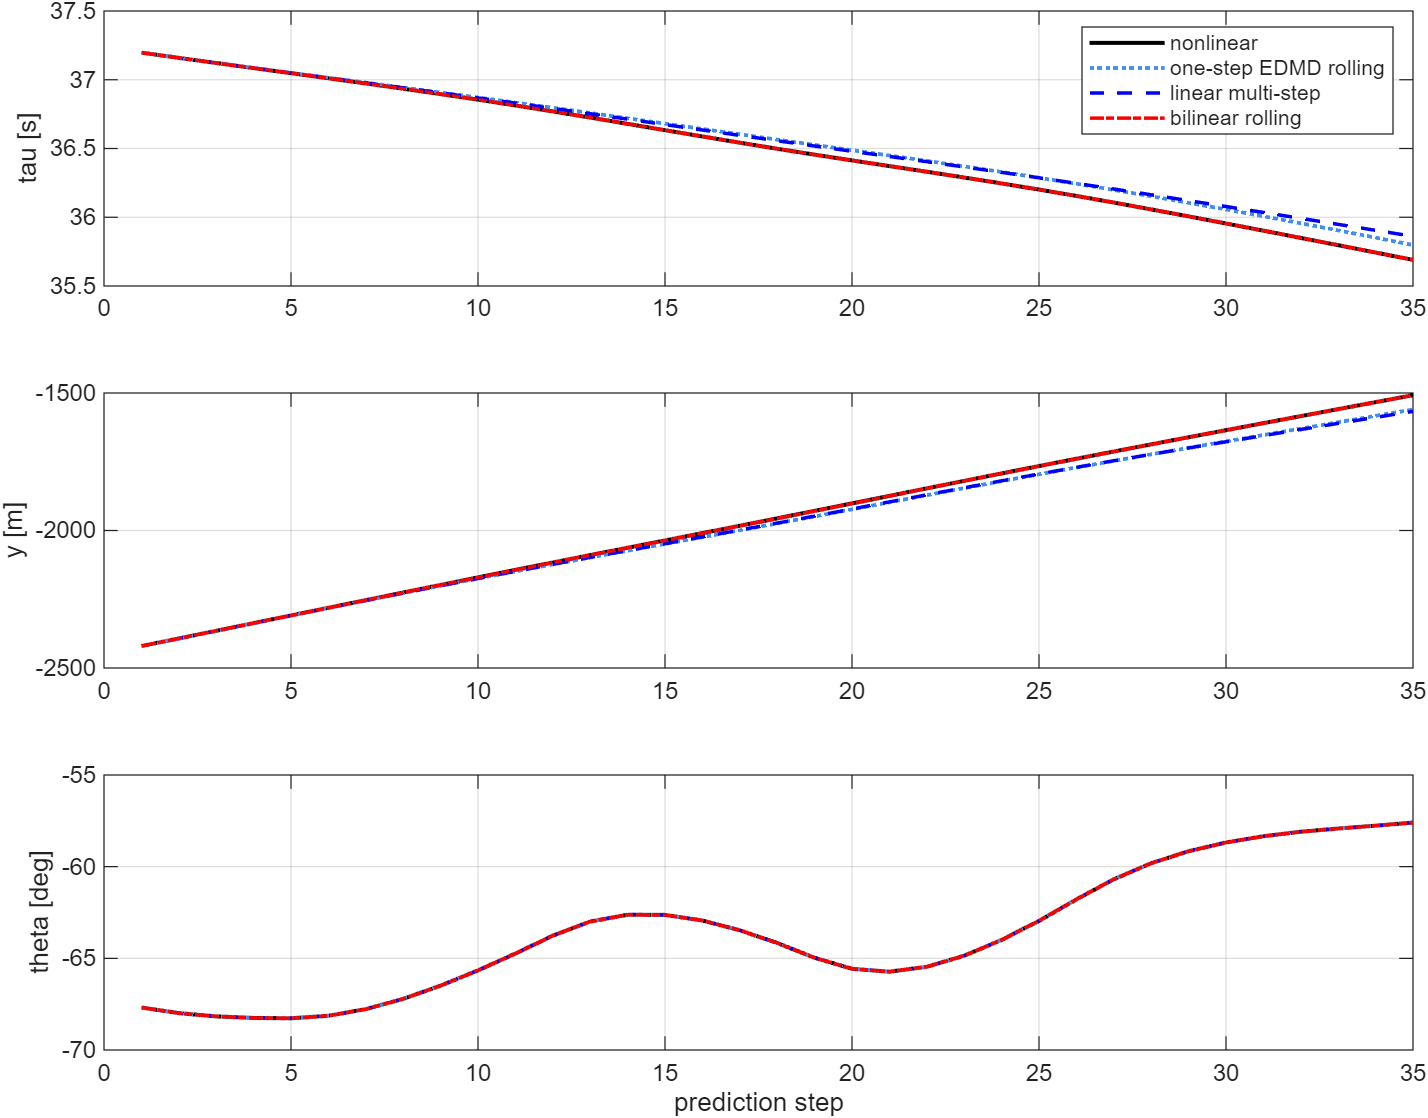
\includegraphics[width=3.35in]{KDPC_RSRFG-main/StationaryTargetKoopman/results/prediction_validation_angle_no_time_dA_5_main.png}
\caption{Prediction comparison for the tuned angle-only run. The bilinear rolling predictor gives substantially lower long-horizon normalized error than rolling one-step EDMD or direct linear multi-step EDMD on the same validation set.}
\label{fig:prediction_angle_only}
\end{figure}

\subsection{Impact-Angle-Constrained Capture Performance}
Table \ref{tab:angle_only_main} reports the main 30$^\circ$ angle-only case with a 5 m capture radius. The nominal case entered the capture set at 37.0 s with a 3.048 m miss distance and a $0.109^\circ$ impact-angle error. The speed-perturbed stress case entered the capture set at 38.0 s with a 4.150 m miss distance and a $0.121^\circ$ angle error. Both cases had no QP failures.

\begin{table}[!t]
\caption{Main 30$^\circ$ Angle-Only Case With 5 m Capture Radius}
\label{tab:angle_only_main}
\centering
\begin{tabular}{c c c c c}
\hline
Case & Captured & Impact time & Miss & Angle error\\
\hline
Nominal & Yes & 37.0 s & 3.048 m & $0.109^\circ$\\
Stress & Yes & 38.0 s & 4.150 m & $0.121^\circ$\\
\hline
\end{tabular}
\end{table}

\begin{figure}[!t]
\centering
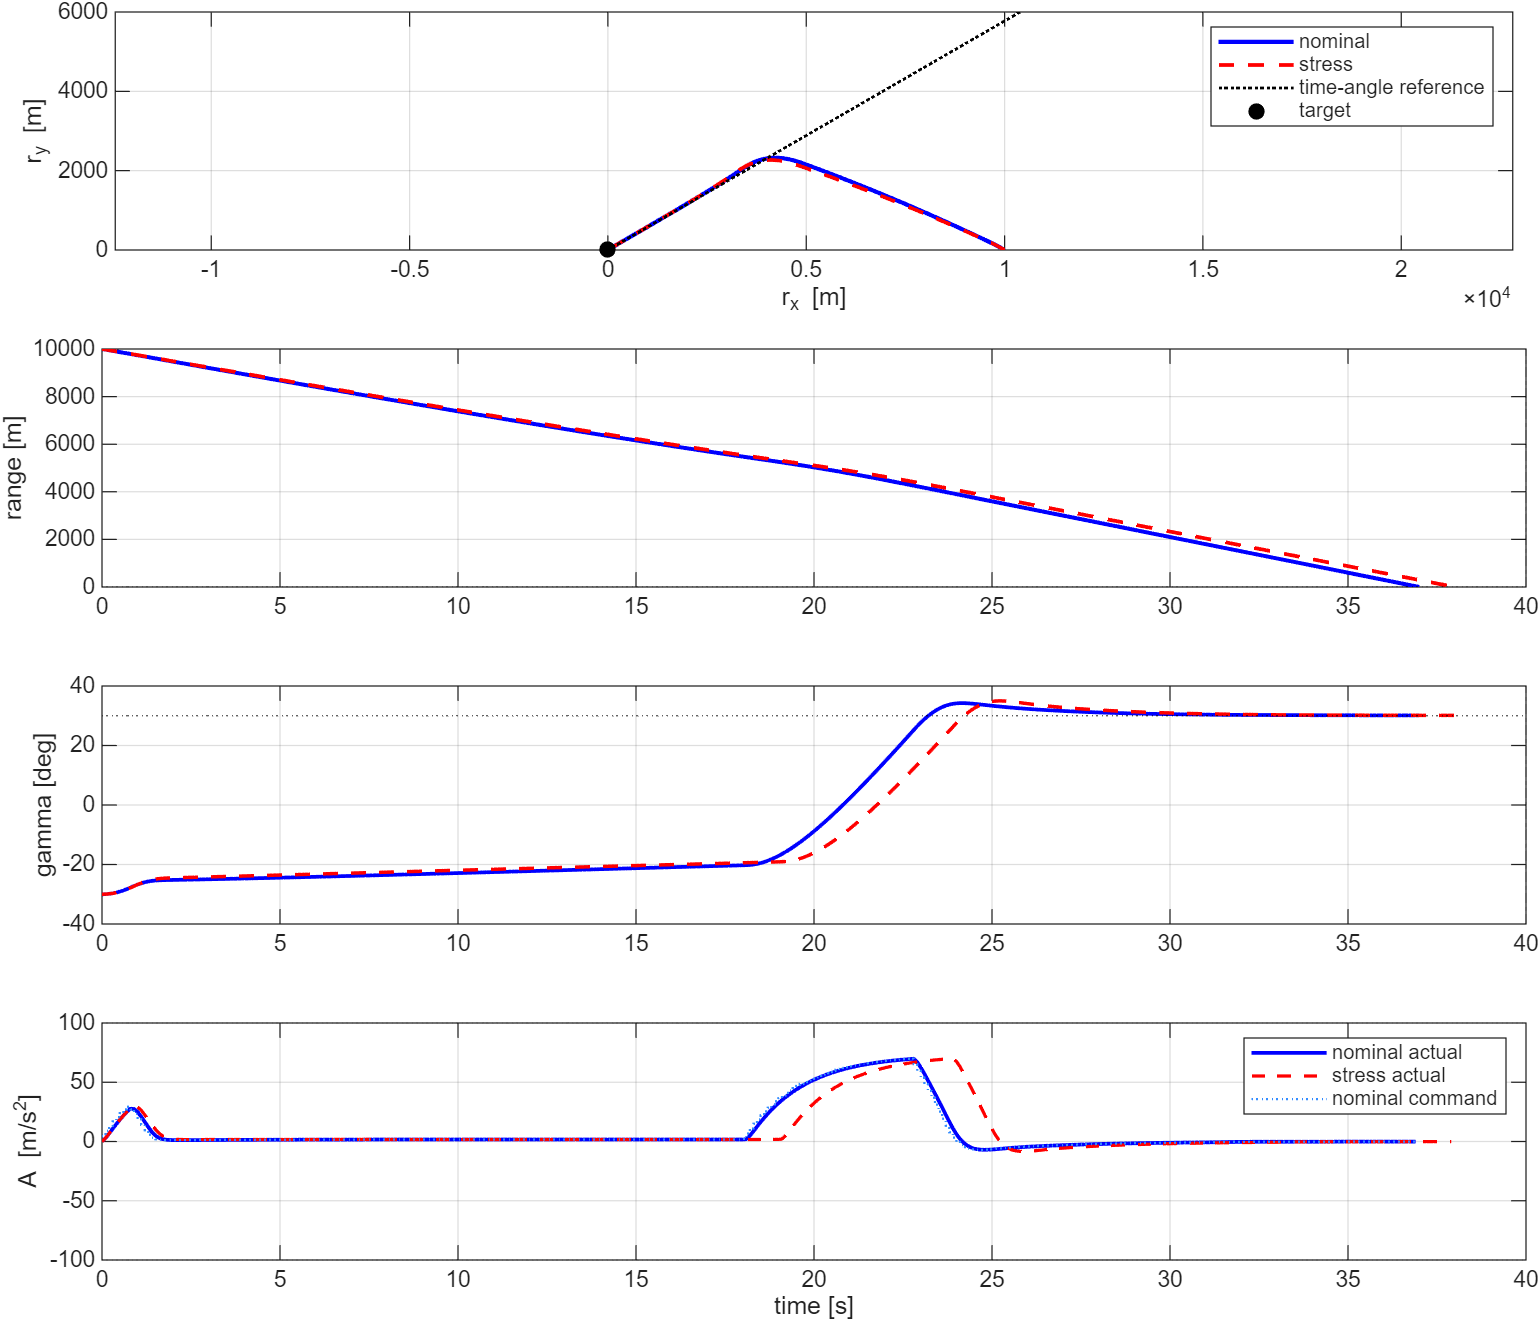
\includegraphics[width=3.35in]{KDPC_RSRFG-main/StationaryTargetKoopman/results/closed_loop_angle_no_time_dA_5_main.png}
\caption{Closed-loop trajectory, range history, heading response, and lateral acceleration for the tuned 30$^\circ$ angle-only case. The actual impact time is an output of the closed-loop trajectory rather than a prescribed terminal constraint.}
\label{fig:closed_loop_angle_only}
\end{figure}

Fig. \ref{fig:closed_loop_angle_only} shows that the trajectory reaches the target neighborhood while aligning the heading with the desired impact direction. The command and first-order-autopilot acceleration remain smooth because the input-difference penalty and acceleration-change bound suppress high-frequency command variation.

\paragraph{Nominal 30$^\circ$ and 45$^\circ$ cases:}
The earlier nominal angle-only tests used a 10 m capture radius and did not prescribe terminal time. Table \ref{tab:angle_only_nominal} reports that both the 30$^\circ$ and 45$^\circ$ commands satisfied the capture and impact-angle requirements. The actual impact times were 22.1 s and 22.9 s, respectively.

\begin{table}[!t]
\caption{Nominal Impact-Angle-Only Cases With 10 m Capture Radius}
\label{tab:angle_only_nominal}
\centering
\begin{tabular}{c c c c}
\hline
$\gamma_f$ & Impact time & Miss & Angle error\\
\hline
30$^\circ$ & 22.1 s & 6.945 m & $-0.107^\circ$\\
45$^\circ$ & 22.9 s & 7.280 m & $-0.404^\circ$\\
\hline
\end{tabular}
\end{table}

\begin{figure*}[!t]
\centering
\subfloat[30$^\circ$ impact-angle command.]{
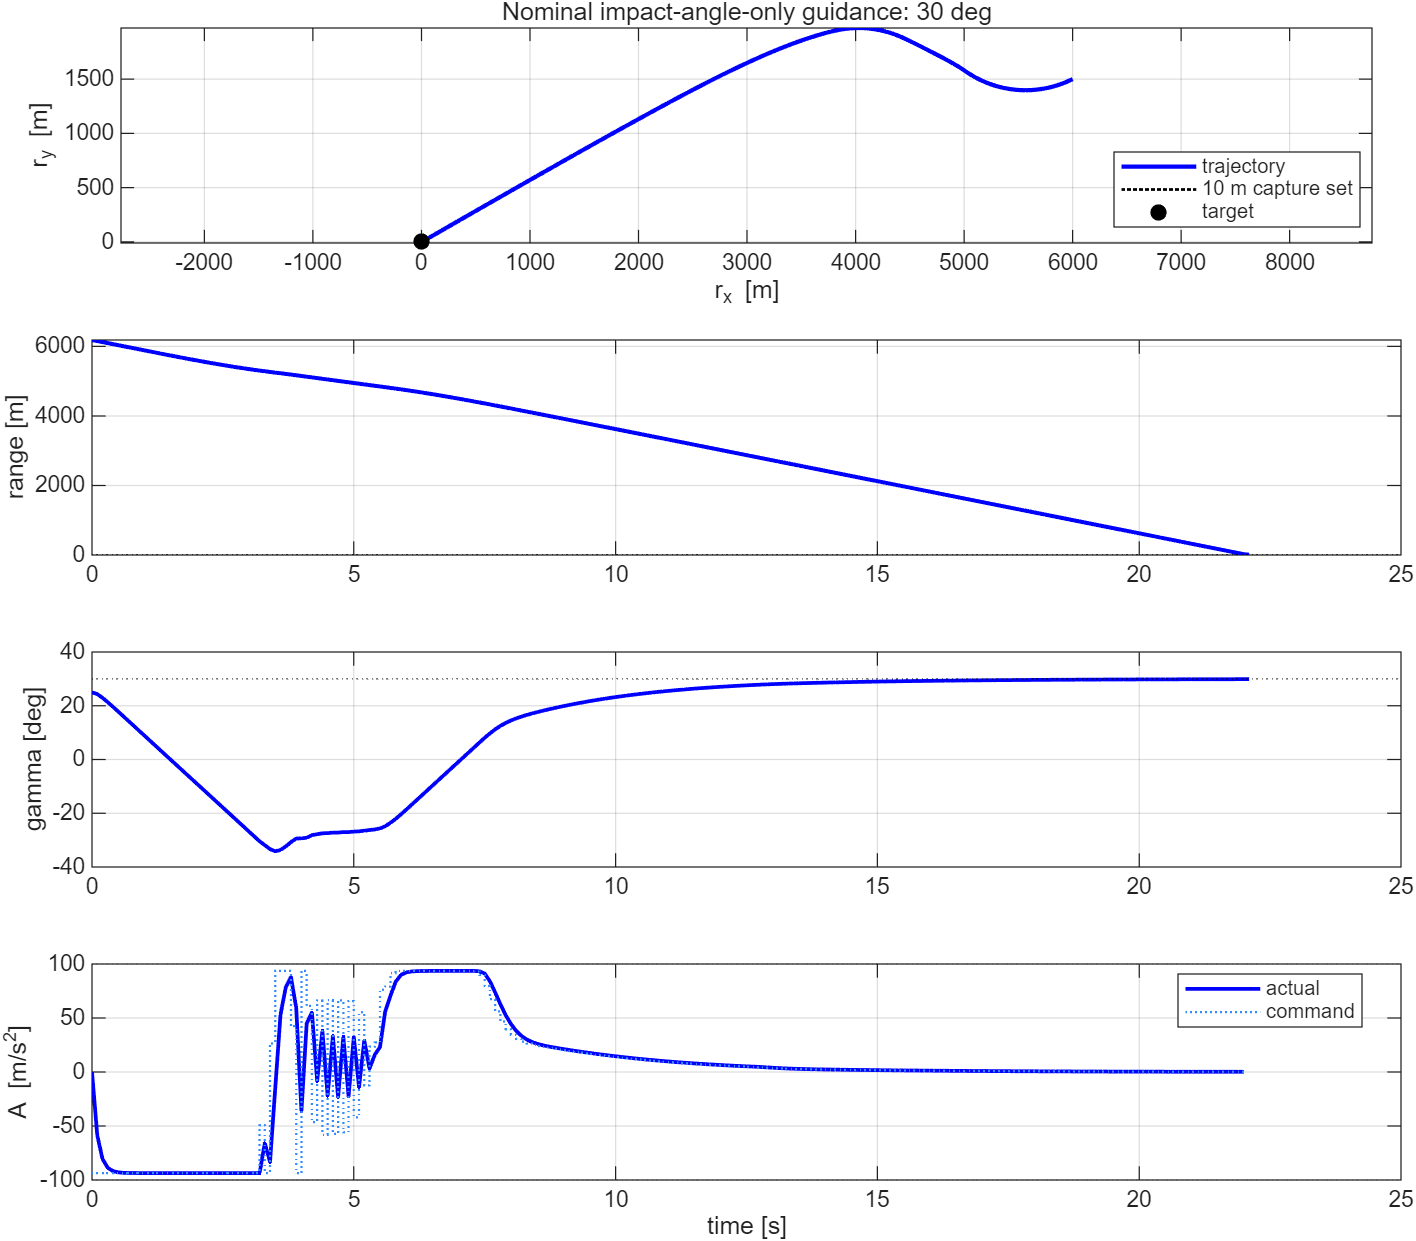
\includegraphics[width=3.35in]{KDPC_RSRFG-main/StationaryTargetKoopman/results/closed_loop_angle_30_nominal.png}}
\hfil
\subfloat[45$^\circ$ impact-angle command.]{
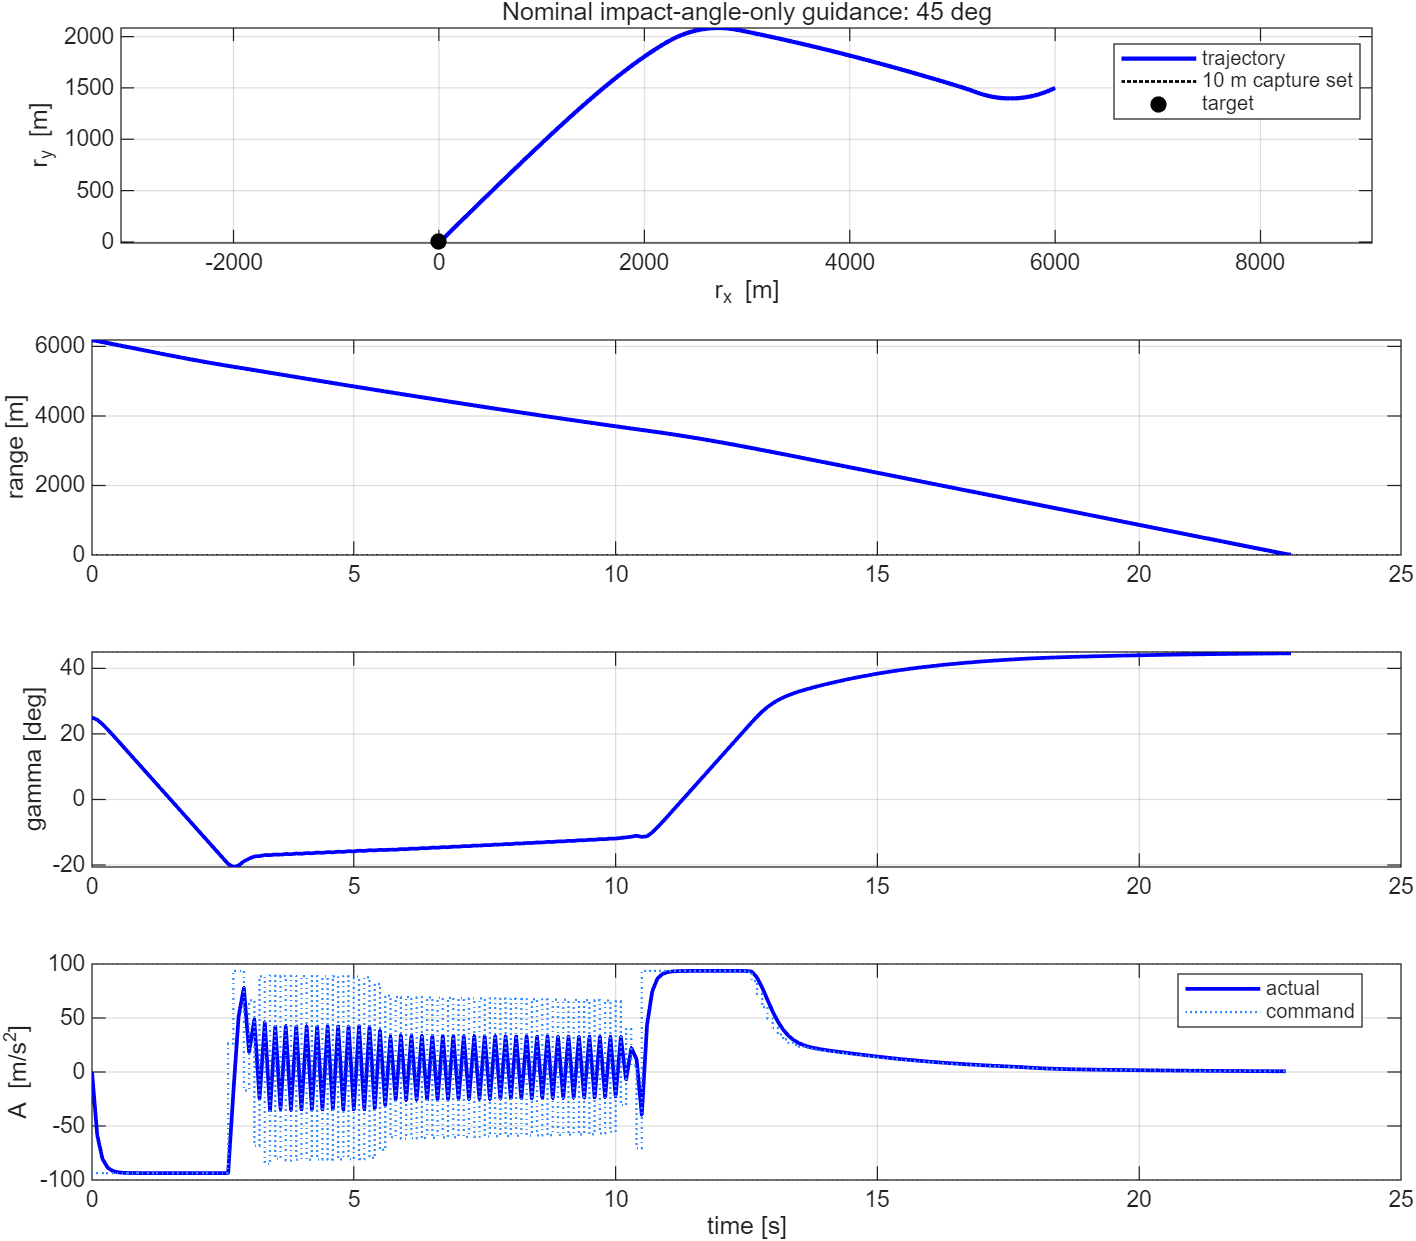
\includegraphics[width=3.35in]{KDPC_RSRFG-main/StationaryTargetKoopman/results/closed_loop_angle_45_nominal.png}}
\caption{Nominal angle-only flight simulations for 30$^\circ$ and 45$^\circ$ impact-angle commands. Both cases satisfy the 10 m capture-radius condition and the 3$^\circ$ impact-angle tolerance without prescribing impact time.}
\label{fig:angle_only_nominal}
\end{figure*}

\subsection{Acceleration-Change Constraint Scan}
The acceleration-change constraint was scanned to examine the role of command smoothing. Table \ref{tab:accel_scan} shows that an intermediate value, $\Delta A_{\max}=5$ m/s$^2$, gave the best nominal and stress capture performance in this set. Removing the constraint caused larger acceleration variation and did not satisfy the 5 m nominal capture requirement. Over-tightening the constraint also degraded capture performance by limiting terminal maneuverability.

\begin{table*}[!t]
\caption{Acceleration-Change Constraint Scan for the 30$^\circ$ Angle-Only Case}
\label{tab:accel_scan}
\centering
\begin{tabular}{c c c c c c c}
\hline
$\Delta A_{\max}$ [m/s$^2$] & Nominal captured & Nominal miss [m] & Nominal angle [deg] & Stress captured & Stress miss [m] & QP failures\\
\hline
$\infty$ & No & 13.489 & -0.081 & Yes & 3.213 & 0/0\\
15 & No & 10.755 & -0.086 & No & 10.707 & 0/0\\
10 & No & 8.208 & -0.070 & No & 8.095 & 0/0\\
5 & Yes & 3.048 & 0.109 & Yes & 4.150 & 0/0\\
3 & No & 17.709 & 0.959 & No & 19.816 & 0/0\\
\hline
\end{tabular}
\end{table*}

\begin{figure}[!t]
\centering
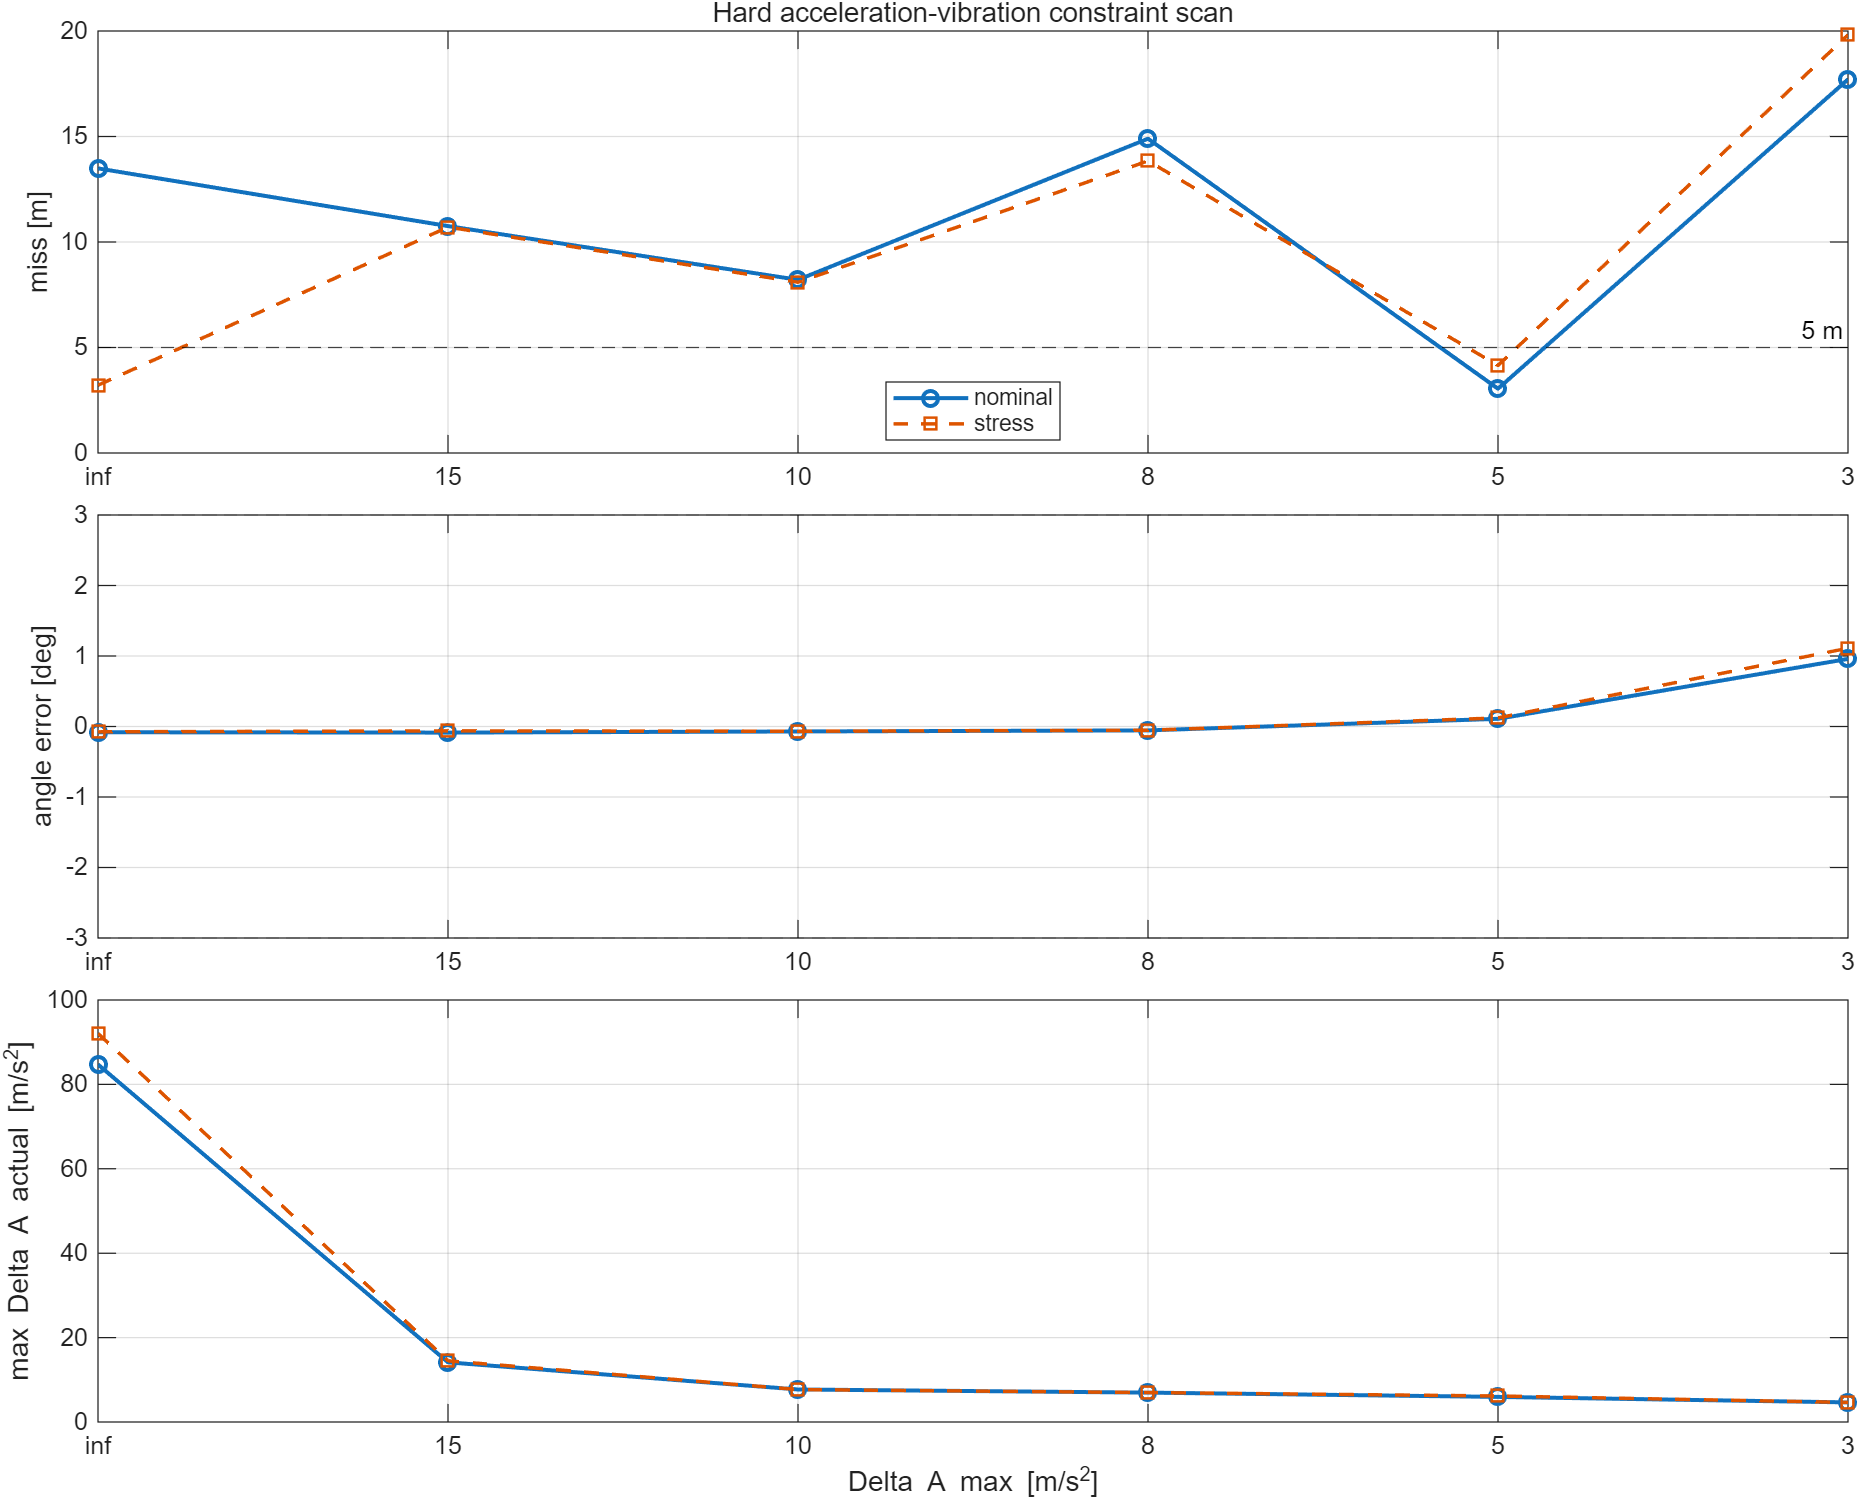
\includegraphics[width=3.35in]{KDPC_RSRFG-main/StationaryTargetKoopman/results/angle_only_accel_vibration_constraint_scan_summary.png}
\caption{Acceleration-change constraint scan. Moderate smoothing improves capture in this tuning set, while either removing the bound or making it too tight degrades the terminal miss distance.}
\label{fig:accel_scan}
\end{figure}

\subsection{Large-Angle Boundary Cases}
Large impact-angle commands expose the current reachable-envelope limitation. A 60$^\circ$ balanced 5 s-horizon case with $\Delta A_{\max}=30$ m/s$^2$ reached 8.187 m nominal miss and $-1.380^\circ$ angle error, but it did not satisfy the stricter 5 m capture requirement and produced many QP failures. A 10 s move-blocking variant reduced trajectory instability relative to unconstrained long-horizon optimization, but still missed the 5 m capture set and produced a larger angle error. These cases indicate that the present angle-only Koopman-MPC design is reliable for moderate impact angles but not yet a complete large-angle guidance solution.

\begin{table}[!t]
\caption{Representative Large-Angle Boundary Cases}
\label{tab:large_angle_boundary}
\centering
\footnotesize
\begin{tabular}{c c c c c}
\hline
Case & Horizon & Miss [m] & Angle error & Failures\\
\hline
60$^\circ$ balanced & 5 s & 8.187 & $-1.380^\circ$ & 163\\
60$^\circ$ move blocking & 10 s & 9.076 & $-9.449^\circ$ & 146\\
80$^\circ$ quick test & 5 s & 11.861 & $-1.285^\circ$ & 290\\
\hline
\end{tabular}
\end{table}

\section{Conclusion}
This paper presented a tube-tightened bilinear Koopman-MPC framework for nominal planar impact-angle guidance without prescribed impact time. The method first formulates a basic capture problem, derives an exact continuous-time bilinear Koopman representation for the ideal stationary-target guidance core, and then extends the terminal output to desired-impact-frame position and heading-error coordinates. The implemented controller combines a task-oriented bilinear EDMD predictor, first-order-autopilot augmentation, sequential convex quadratic programming, terminal slack variables, input-difference regularization, and validation-data residual-tube tightening. In the main 30$^\circ$ angle-only case, the controller achieved a 3.048 m nominal miss distance and a $0.109^\circ$ impact-angle error within a 5 m capture radius; the speed-perturbed stress case also satisfied the capture condition. Nominal 30$^\circ$ and 45$^\circ$ cases satisfied a 10 m capture-radius requirement. Acceleration-rate scans and large-angle tests show that the method remains tuning-sensitive and incomplete for aggressive impact-angle commands. The appropriate conclusion is therefore bounded: removing the fixed impact-time constraint yields a more credible and better-supported Koopman-MPC guidance formulation for the present data and simulations.

\balance
\begin{thebibliography}{99}

\bibitem{koopman1931}
B. O. Koopman, ``Hamiltonian systems and transformation in Hilbert space,'' \emph{Proceedings of the National Academy of Sciences}, vol. 17, no. 5, pp. 315--318, 1931.

\bibitem{williams2015edmd}
M. O. Williams, I. Kevrekidis, and C. Rowley, ``A data-driven approximation of the Koopman operator: Extending dynamic mode decomposition,'' \emph{Journal of Nonlinear Science}, vol. 25, no. 6, pp. 1307--1346, 2015.

\bibitem{korda2018mpc}
M. Korda and I. Mezic, ``Linear predictors for nonlinear dynamical systems: Koopman operator meets model predictive control,'' \emph{Automatica}, vol. 93, pp. 149--160, 2018.

\bibitem{bevanda2021kodm}
P. Bevanda, S. Sosnowski, and S. Hirche, ``Koopman operator dynamical models: Learning, analysis and control,'' \emph{Annual Reviews in Control}, vol. 52, pp. 197--212, 2021.

\bibitem{dejong2024kdpc}
T. de Jong, V. Breschi, M. Schoukens, and M. Lazar, ``Koopman data-driven predictive control with robust stability and recursive feasibility guarantees,'' in \emph{Proc. 63rd IEEE Conference on Decision and Control}, 2024, pp. 140--145.

\bibitem{zhou2024klmpc}
M. Zhou, M. Lu, G. Hu, Z. Guo, and J. Guo, ``Koopman operator-based integrated guidance and control for strap-down high-speed missiles,'' \emph{IEEE Transactions on Control Systems Technology}, vol. 32, no. 6, pp. 2436--2449, 2024.

\end{thebibliography}

\end{document}
